\documentclass[letterpaper,12pt]{article}
\usepackage[utf8]{inputenc}
\makeatletter
\renewcommand{\@seccntformat}[1]{%
  \ifcsname specialformat#1\endcsname
    \csname specialformat#1\endcsname
  \else
    \csname the#1\endcsname\quad % default
  \fi
}
\makeatother
\newcommand{\specialformatsection}{}
\renewcommand{\thesubsection}{\arabic{subsection}}

\usepackage[T1]{fontenc}
\usepackage{charter}
\usepackage{geometry}
\usepackage{amsmath}
\usepackage{float}
\usepackage{graphicx}
\usepackage{subcaption}
\usepackage{amssymb}
\usepackage{adjustbox}
\usepackage{wrapfig} %%imagen envuelta por un texto
\usepackage{xcolor}
\usepackage{fancyhdr}
\usepackage{tabularx} %%TABLAS OH YEAH

\title {\textbf{Análisis del cliente}}
\author{Lara Xocuis Martha Denisse}
\date{23 de noviembre de 2023}
\geometry{top=2cm, bottom=2cm, left=2cm, right= 2cm} %%margen
\graphicspath{{images/}}
\parindent=0pt

\begin{document}
\maketitle
\newpage
%%%%%%%%%%%%%%%%%%%%%%%%%%%%%%%%%%%%%%%%%%%%%%%%%%%%%%%%%%%%%%%%%%%%%%%%%%%%
\begin{sloppypar}
\section{Introducción}
Se entrevistaron a siete personas con la finalidad de conocer si el cliente está satisfecho con las instalaciones que tiene su niño, así como la atención, cuidado, seguridad, orientación y aprendizaje. Al participar en esta encuesta, los clientes no solo comparten su perspectiva individual, sino que también contribuyen al continuo esfuerzo de mejora y excelencia en los servicios. \textit{Los resultados obtenidos serán analizados de manera confidencial y se utilizarán para identificar áreas de fortaleza y oportunidades de mejora.}
\vspace{0.3cm}\\ 
Se explorará en detalle los resultados obtenidos, destacando áreas de satisfacción y áreas que pueden beneficiarse de ajustes y mejoras. Cada respuesta aportada en la encuesta es de suma importancia ya que nos brinda una visión única de la experiencia individual de cada familia en nuestra guardería.
\newpage
\section{Análisis de las respuestas}
La encuesta, distribuida entre los padres de la guardería, constaba de preguntas estructuradas que abordaban temas específicos relacionados con la calidad de los servicios ofrecidos. La participación fue voluntaria y anónima para garantizar la sinceridad y la objetividad en las respuestas. 

\subsubsection{Pregunta por pregunta}
\begin{enumerate}
  \item Del 1 al 5, ¿qué tan satisfech@ se siente con las instalaciones para su(s) hijo(s)?
  \begin{figure}[H]
    \centering 
    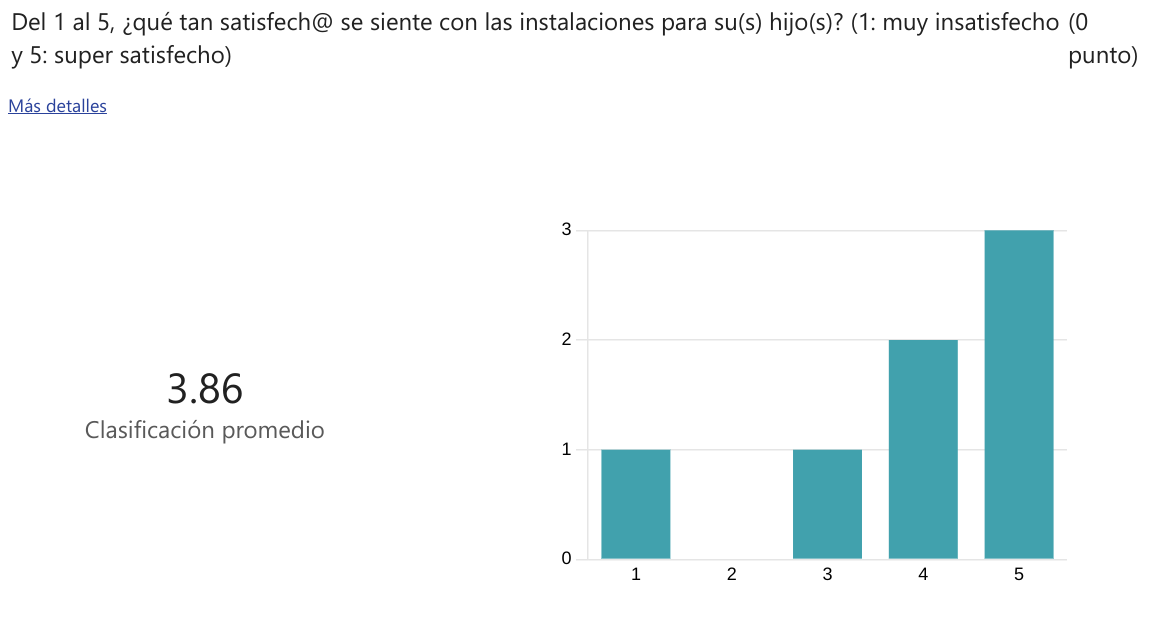
\includegraphics[width=0.6\textwidth]{1.png}
  \end{figure}
  De acuerdo a la gráfica y a su calificación promedio (3.86), se puede decir que la mayoría de las personas si se siente satisfecho con las instalaciones.
  \item Del 1 al 5, ¿cree que el ambiente de la guardería es el adecuado para su(s) hijo(s)? 
  \begin{figure}[H]
    \centering 
    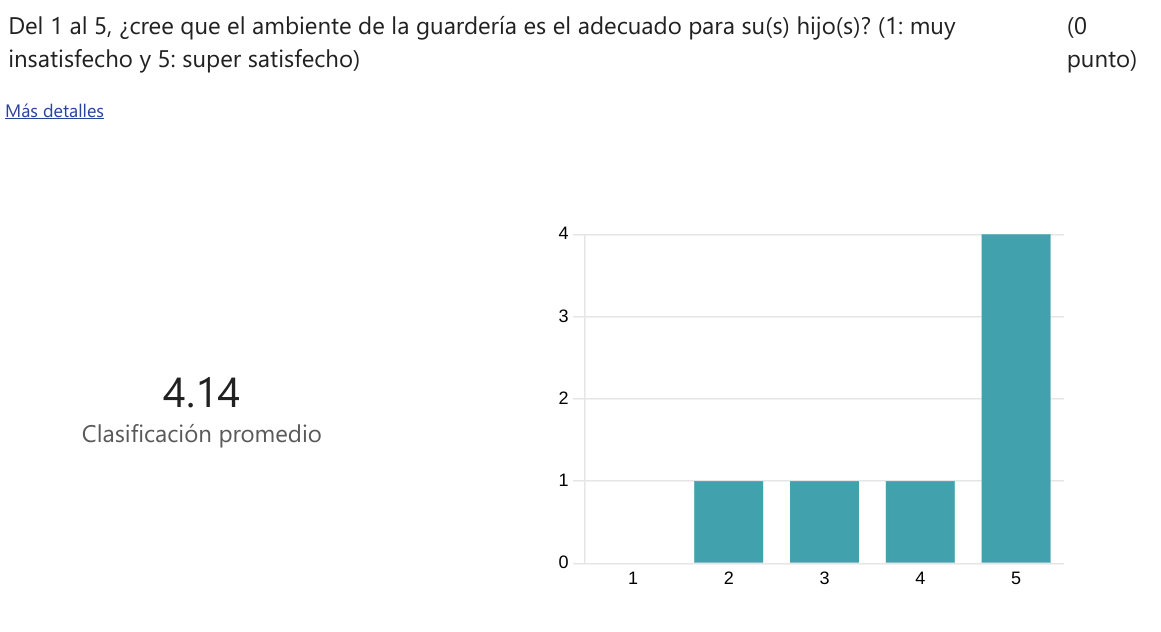
\includegraphics[width=0.6\textwidth]{2.png}
  \end{figure}
  De acuerdo a el gráfico, la mayoría de las personas sí cree que el ambiente de la guardería es adecuado.
  \newpage
  \item Del 1 al 5, ¿qué tan importante cree usted en los protocolos de seguridad que impone la guardería para el cuidado de su(s) hijo(s)? 
  \begin{figure}[H]
    \centering 
    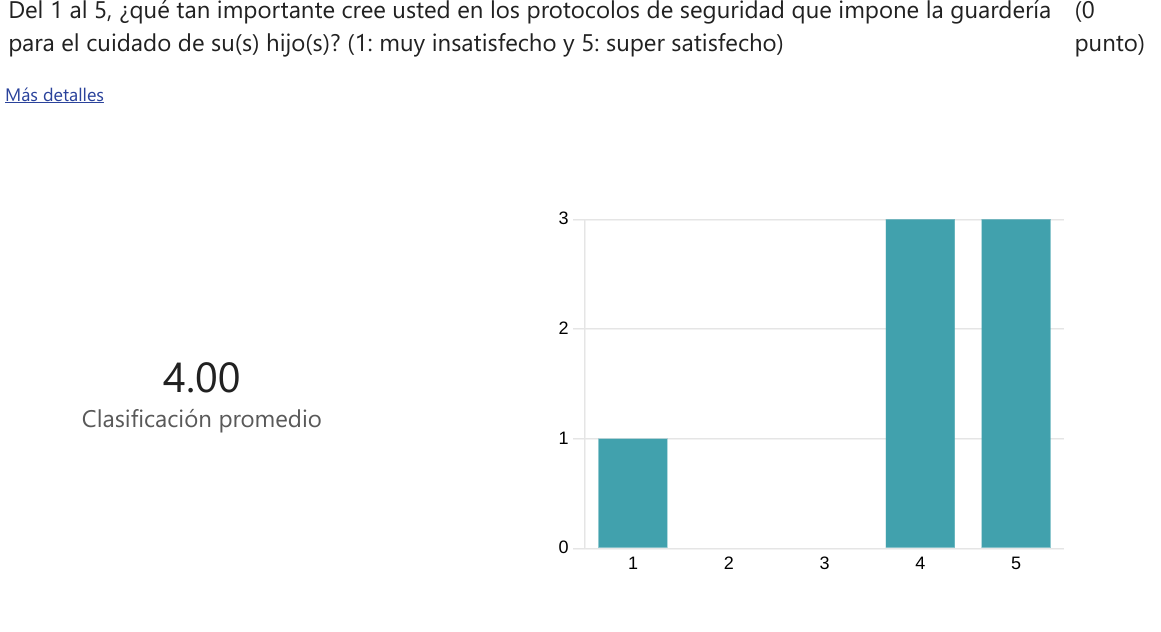
\includegraphics[width=0.6\textwidth]{3.png}
  \end{figure}
  De acuerdo a los resultados, la mayoría de las personas tiene una buena perspectiva con los protocolos de seguridad de la guardería en relación del cuidado del niño.
  \item Del 1 al 5, ¿qué tan satisfech@ se siente con la atención al cliente? 
  \begin{figure}[H]
    \centering 
    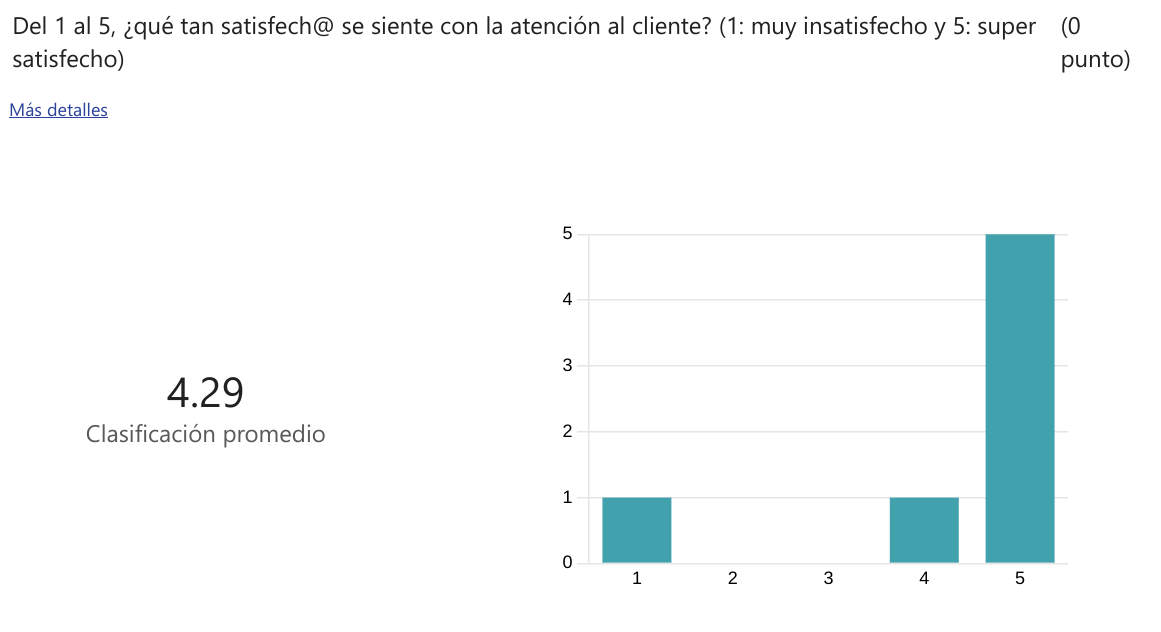
\includegraphics[width=0.6\textwidth]{4.png}
  \end{figure}
  La mayoria (por no decir todos) están satisfechos con la atención al cliente.
  \newpage
  \item Del 1 al 5, ¿qué tan satisfech@ se siente con las actividades para su(s) hijo(s) dentro de la guardería? 
  \begin{figure}[H]
    \centering 
    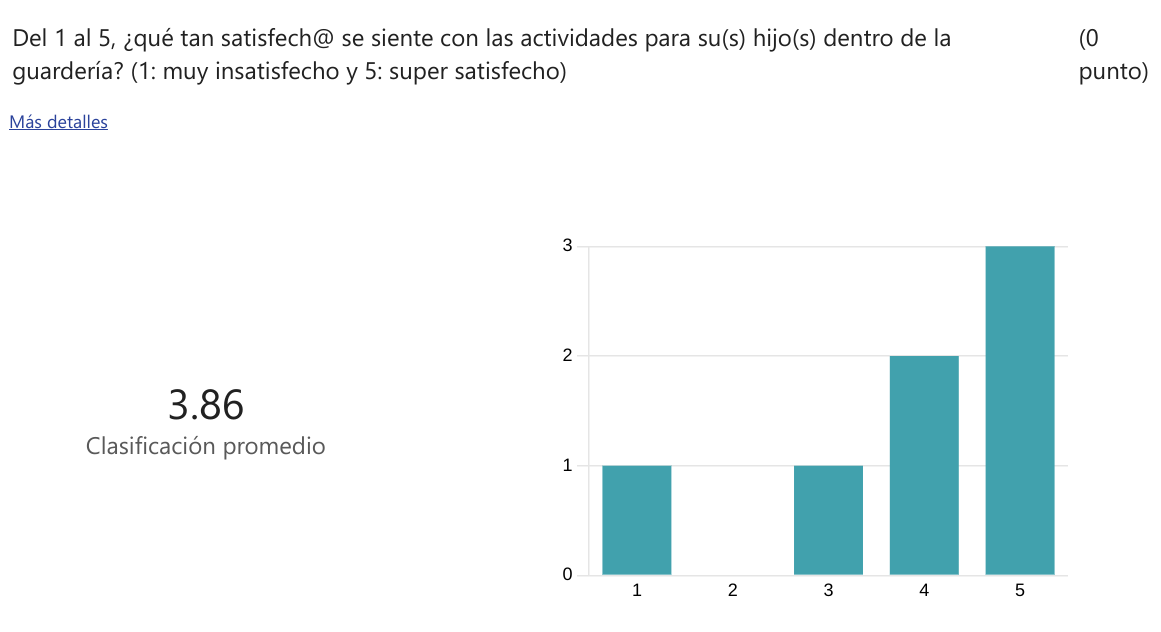
\includegraphics[width=0.6\textwidth]{5.png}
  \end{figure}
  De cierta forma, casi todas las personas se sienten satisfechas con las actividades para sus hijos.
  \item Del 1 al 5, ¿qué tan satisfech@ se siente con la orientación para su(s) hijo(s) dentro de la guardería? 
  \begin{figure}[H]
    \centering 
    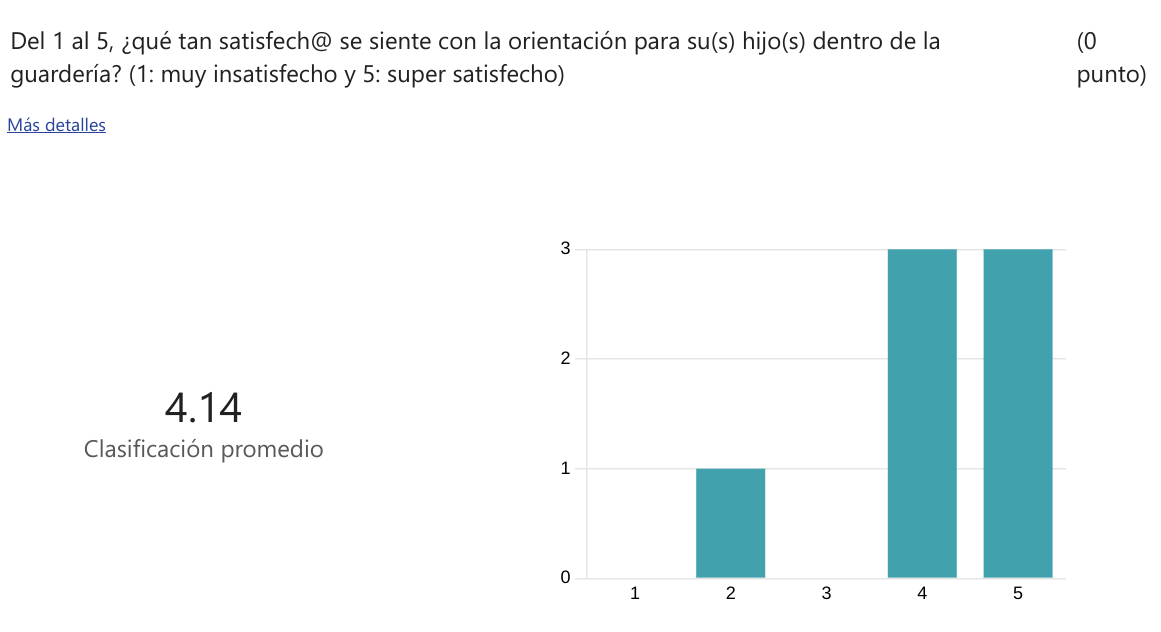
\includegraphics[width=0.6\textwidth]{6.png}
  \end{figure}
  La mayoría de personas se sienten satisfechos con la orientación de los niños.
  \newpage
  \item Del 1 al 5, ¿qué tan satisfech@ se siente con la organización de la guardería? 
  \begin{figure}[H]
    \centering 
    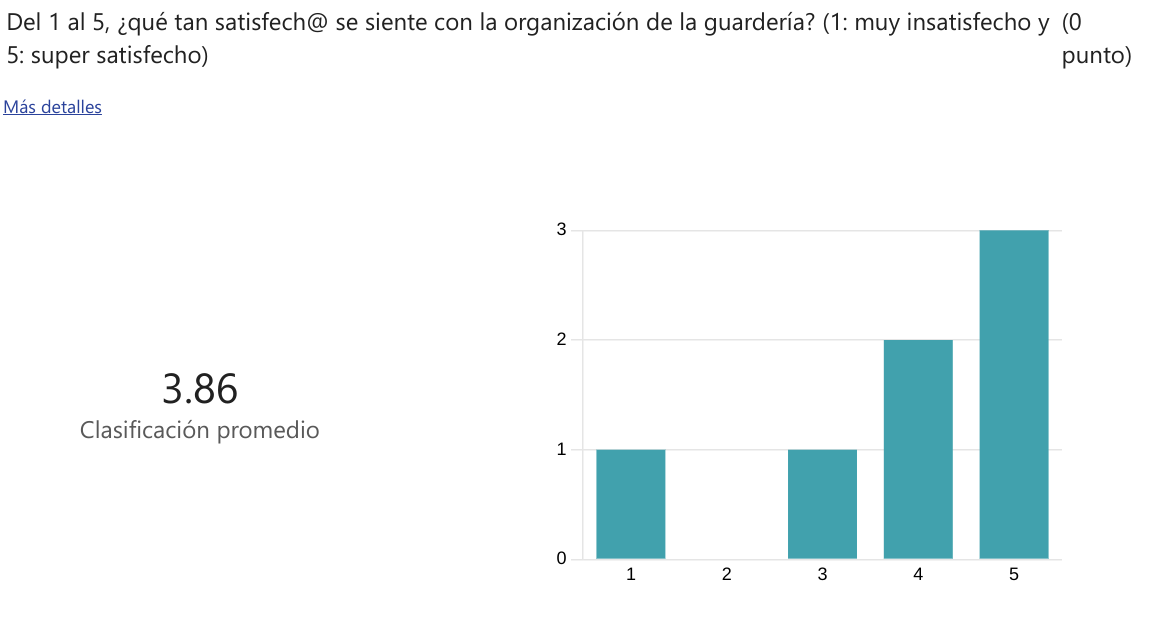
\includegraphics[width=0.6\textwidth]{7.png}
  \end{figure}
  De acuerdo a la gráfica, casi la mayoría de personas se sienten satisfechos con la organización de la guardería.
  \item Del 1 al 5, ¿qué tan satisfech@ se siente con el proceso de inscripción para su(s) hijo(s)? 
  \begin{figure}[H]
    \centering 
    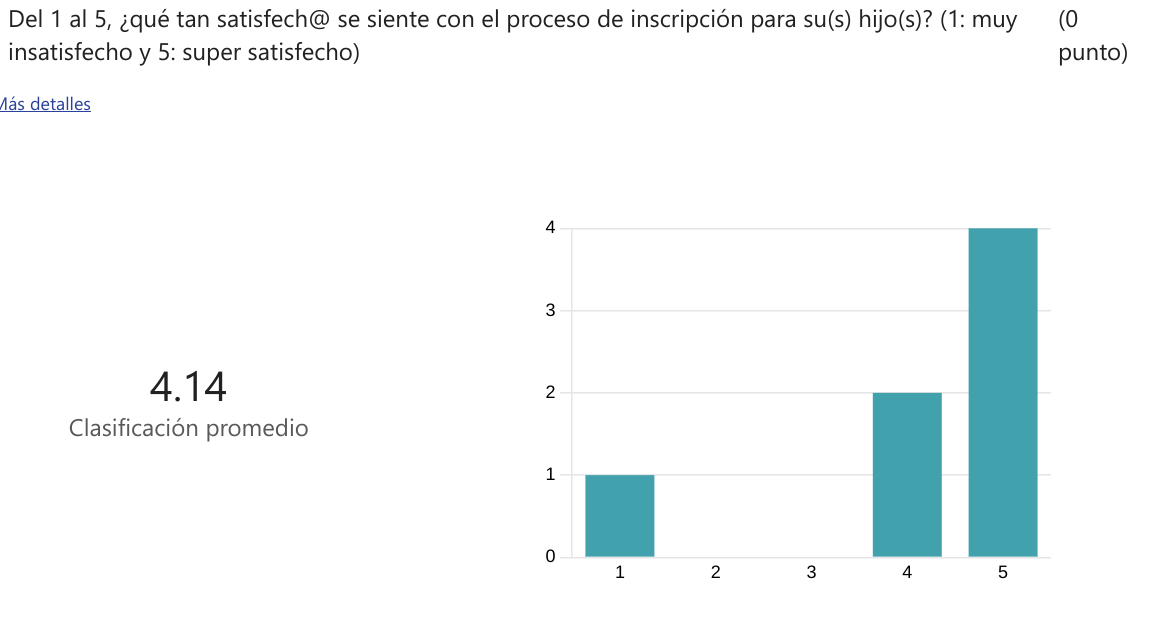
\includegraphics[width=0.6\textwidth]{8.png}
  \end{figure}
  El gráfico anterior hace demostrar que la mayoría de personas se siente satisfecha con el proceso de inscripción.
  \item Del 1 al 5, ¿qué tan satisfech@ se siente de la atención que recibió? 
  \begin{figure}[H]
    \centering 
    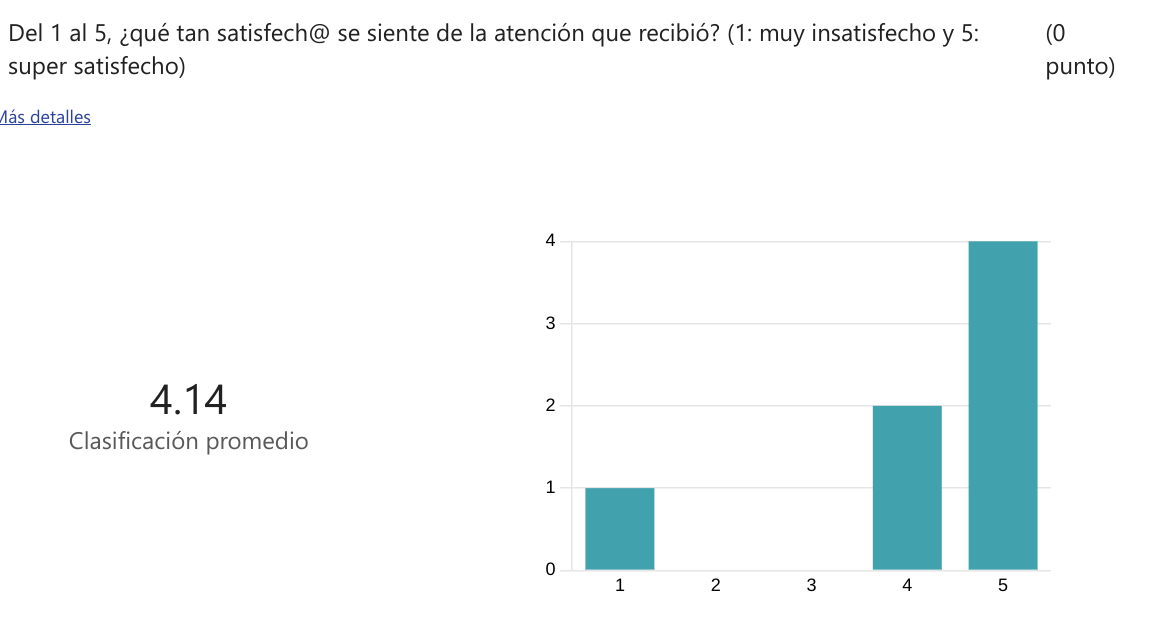
\includegraphics[width=0.6\textwidth]{9.png}
  \end{figure}
  La mayoría de personas se siente satisfecha con la atención recibida.
  \item ¿Ha recomendado nuestros servicios a otras personas?
  \begin{figure}[H]
    \centering 
    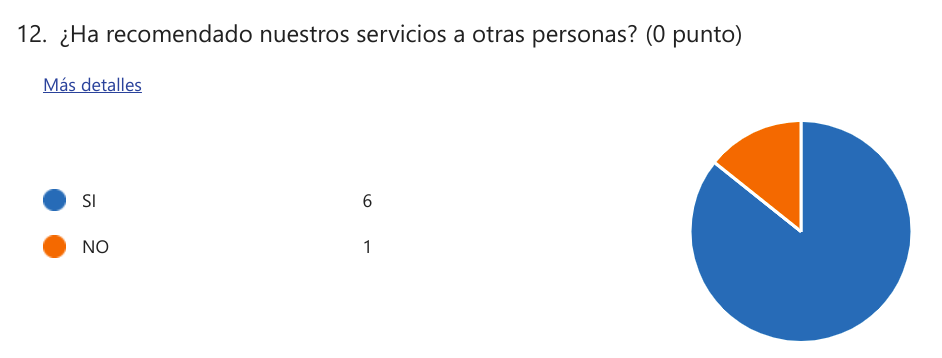
\includegraphics[width=0.6\textwidth]{10.png}
  \end{figure}
  La mayoría ha recomendado el servicio de guardería.
  \item ¿Qué opina sobre el precio de inscripción? ¿Cree que es adecuado?. Escriba un comentario breve
  \begin{figure}[H]
    \centering 
    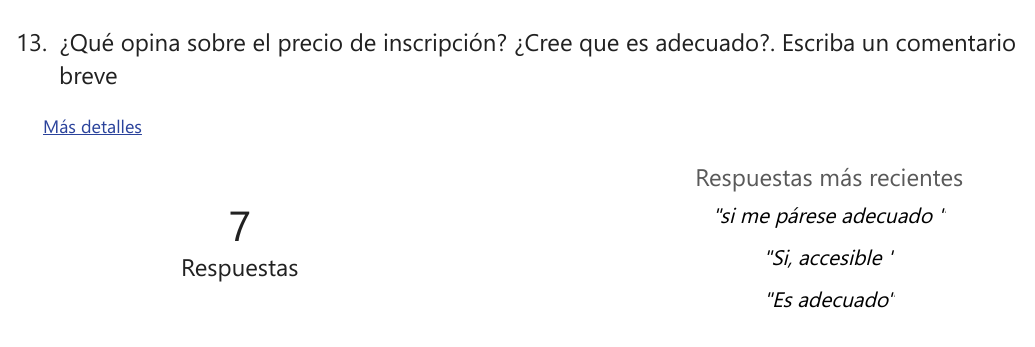
\includegraphics[width=0.6\textwidth]{11.png}
  \end{figure}
  Opiniones positivas sobre el precio de inscripción.
  \item ¿Qué áreas considera que deberíamos mejorar?
  \begin{figure}[H]
    \centering 
    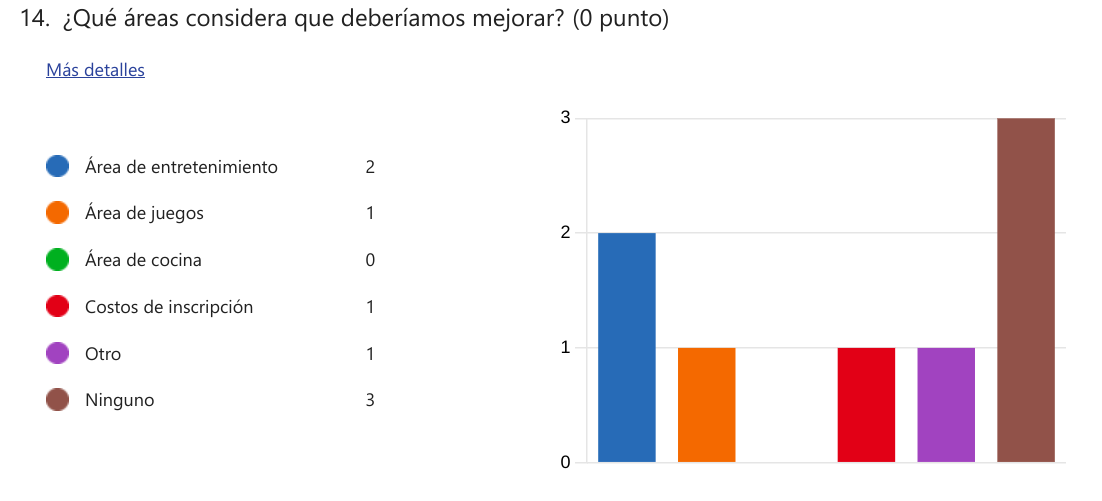
\includegraphics[width=0.6\textwidth]{12.png}
  \end{figure}
  La mayoría considera que no es necesario mejorar nada en la guardería.
  \item ¿Qué es lo que más le gusta de nuestros servicios?
  \begin{figure}[H]
    \centering 
    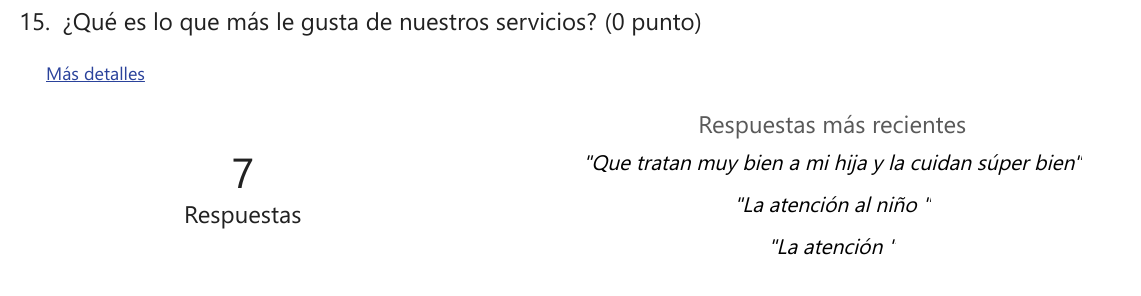
\includegraphics[width=0.6\textwidth]{13.png}
  \end{figure}
  A muchos clientes les gusta el trato y atención al niño de sus hijos.
  \item ¿Ha tenido alguna mala experiencia dentro de la guardería? Si es así, ¿cuál fue?
  \begin{figure}[H]
    \centering 
    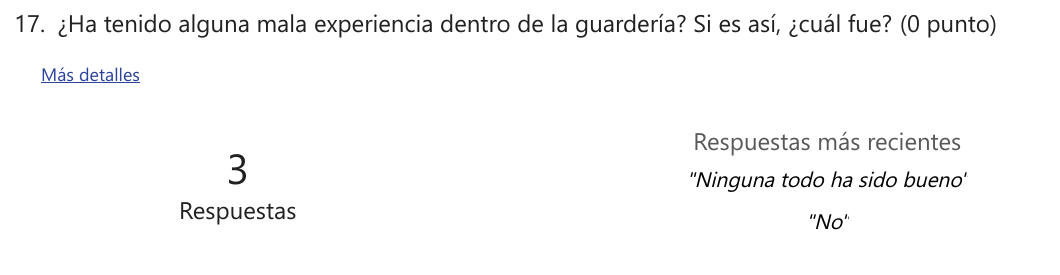
\includegraphics[width=0.6\textwidth]{14.png}
  \end{figure}
  No se registran malas experiencias dentro de la guardería.
\end{enumerate}
\subsubsection{Conclusión} 
Los resultados indican una satisfacción general de los padres en múltiples aspectos de la experiencia en la guardería "Ternutira de mamá".
\vspace{0.3cm}\\ 
El análisis detallado de los resultados de la encuesta demuestra una satisfacción significativa con las instalaciones, la atención y cuidado brindado, la seguridad percibida, la orientación proporcionada y los programas de aprendizaje ofrecidos.
\vspace{0.3cm}\\ 
Las áreas de fortaleza identificadas, como la alta calificación de instalaciones y la satisfacción con la atención personalizada, son testimonios positivos del compromiso y dedicación del personal de la guardería.
\vspace{0.3cm}\\ 
\textbf{Es importante destacar que, a pesar de que muchos padres no pudieron participar en dicha en cuesta por falta de tiempo, han declarado su fuerte gusto por los tratos de la guardería. }

\subsubsection{Sugerencias (estrategias)}
Algunas de las estrategias pueden ser en fortalecer la comunicación y medidas de seguridad, estas ofrecen una dirección clara para fortalecer aún más la relación entre la guardería y los padres. Estas estrategias no solo abordan áreas de mejora señaladas por los padres, sino que también refuerzan la transparencia y colaboración en beneficio de la comunidad.
\vspace{0.3cm}\\ 
Se refuerza la idea de que la participación activa de los padres es esencial para el éxito continuo de la guardería. La colaboración entre la administración, el personal y las familias hace que la guardería pueda avanzar de manera óptima y que el niño se sienta seguro dentro de dicha instalación.

\section{Conclusión Personal}
Este proceso de análisis destaca la importancia de escuchar activamente a nuestra comunidad de padres. Sus opiniones no solo guían las acciones de la guardería, sino que también refuerzan el vínculo de confianza entre la guardería y las familias. La búsqueda de la excelencia en el cuidado y educación infantil se fortalece con cada respuesta compartida.

\section{Aprendizaje}
Este informe y análisis reitera la importancia de la retroalimentación de los padres de los niños para la mejora continua entre el servicio de la guardería. Orienta de gran manera las estrategias para brindar un ambiente necesario para el desarrollo de los niños.

\section{Anexos}
cuestionario en blanco blalbal
\begin{figure}[H]
  \centering 
  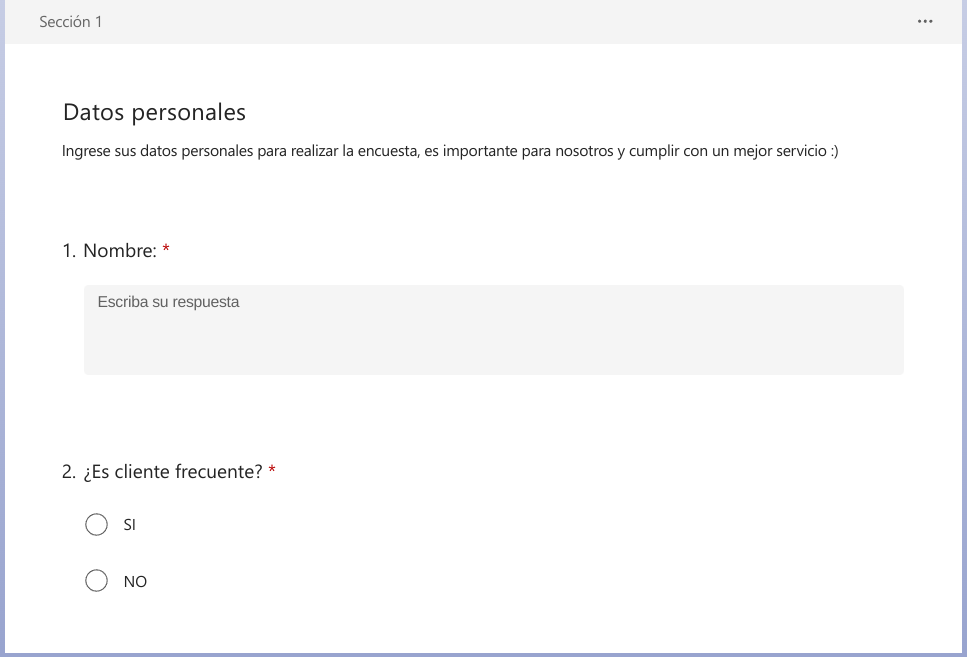
\includegraphics[width=0.9\textwidth]{gestionalanilis.png}
  \caption{Retención de clientes}
\end{figure}
\begin{figure}[H]
  \centering 
  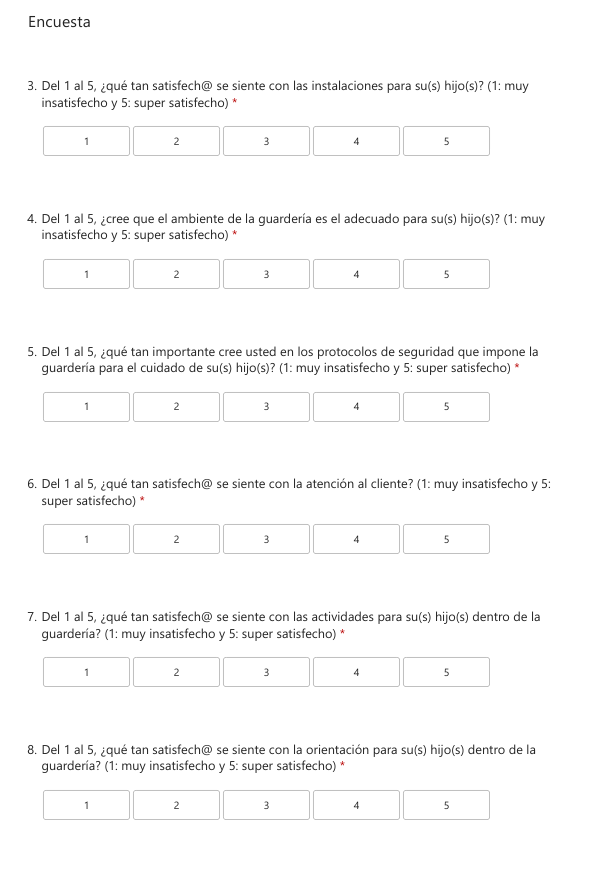
\includegraphics[width=0.9\textwidth]{ges1.png}
\end{figure}
\begin{figure}[H]
  \centering 
  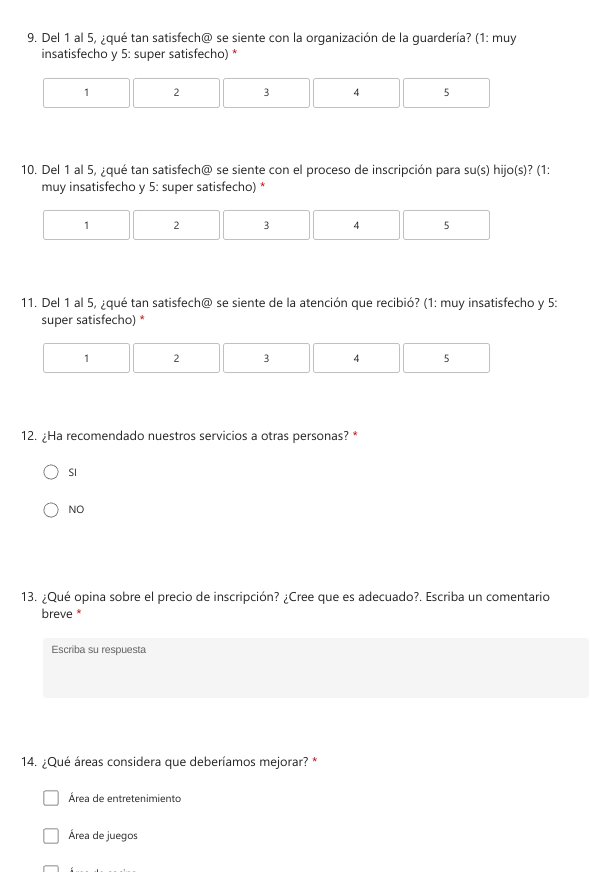
\includegraphics[width=0.9\textwidth]{ges2.png}
\end{figure}
\begin{figure}[H]
  \centering 
  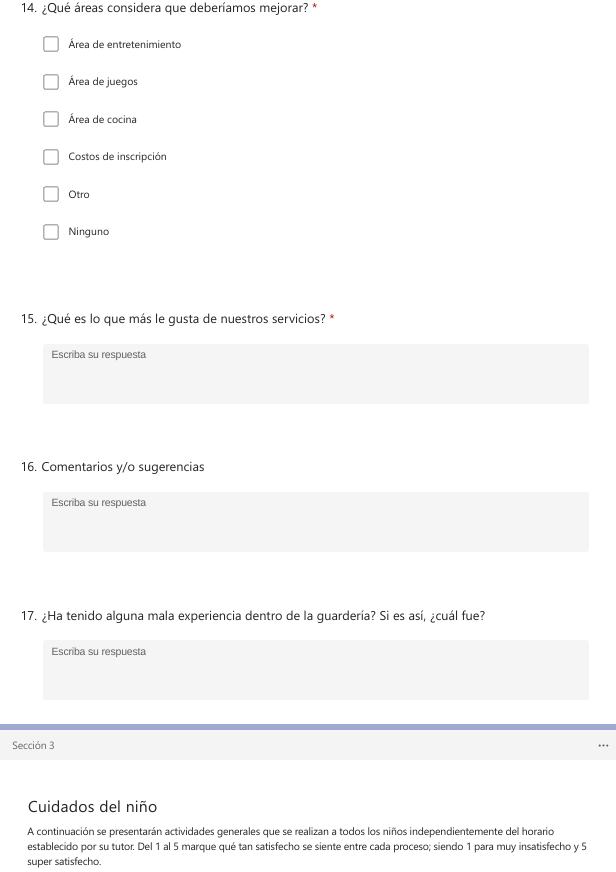
\includegraphics[width=0.9\textwidth]{ges3.png}
\end{figure}
\begin{figure}[H]
  \centering 
  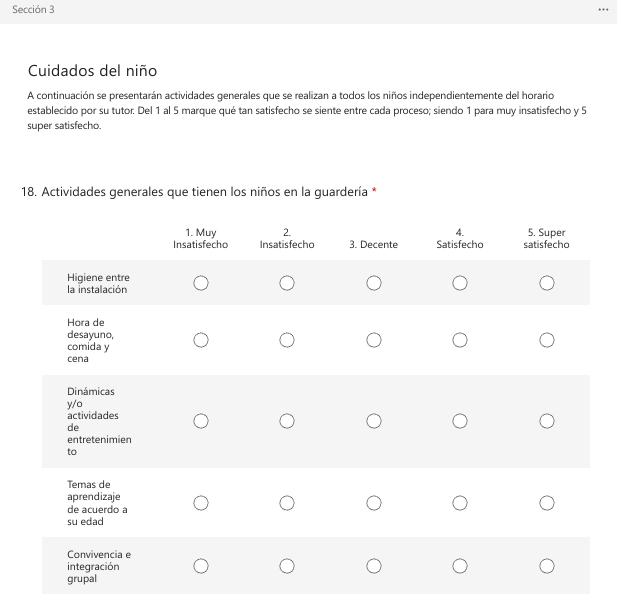
\includegraphics[width=0.9\textwidth]{ges4.png}
\end{figure}
\begin{figure}[H]
  \centering 
  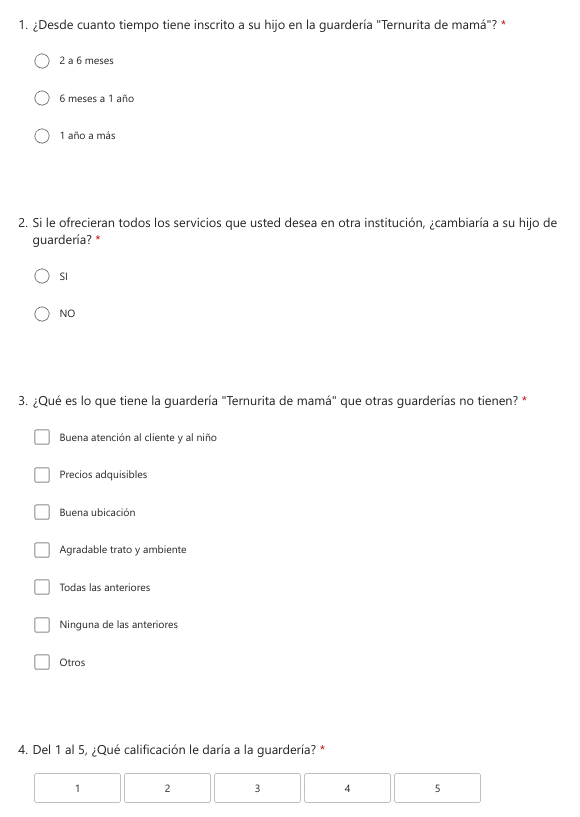
\includegraphics[width=0.9\textwidth]{gestion5.png}
  \caption{Lealtad de clientes}
\end{figure}

\end{sloppypar}
\end{document}